\documentclass{article}
\usepackage{amsmath,amssymb}
\usepackage{fullpage}
\usepackage{graphicx}

\newcommand{\mudn}{\mu_\downarrow}
\newcommand{\muup}{\mu_\uparrow}

\begin{document}

\begin{center}
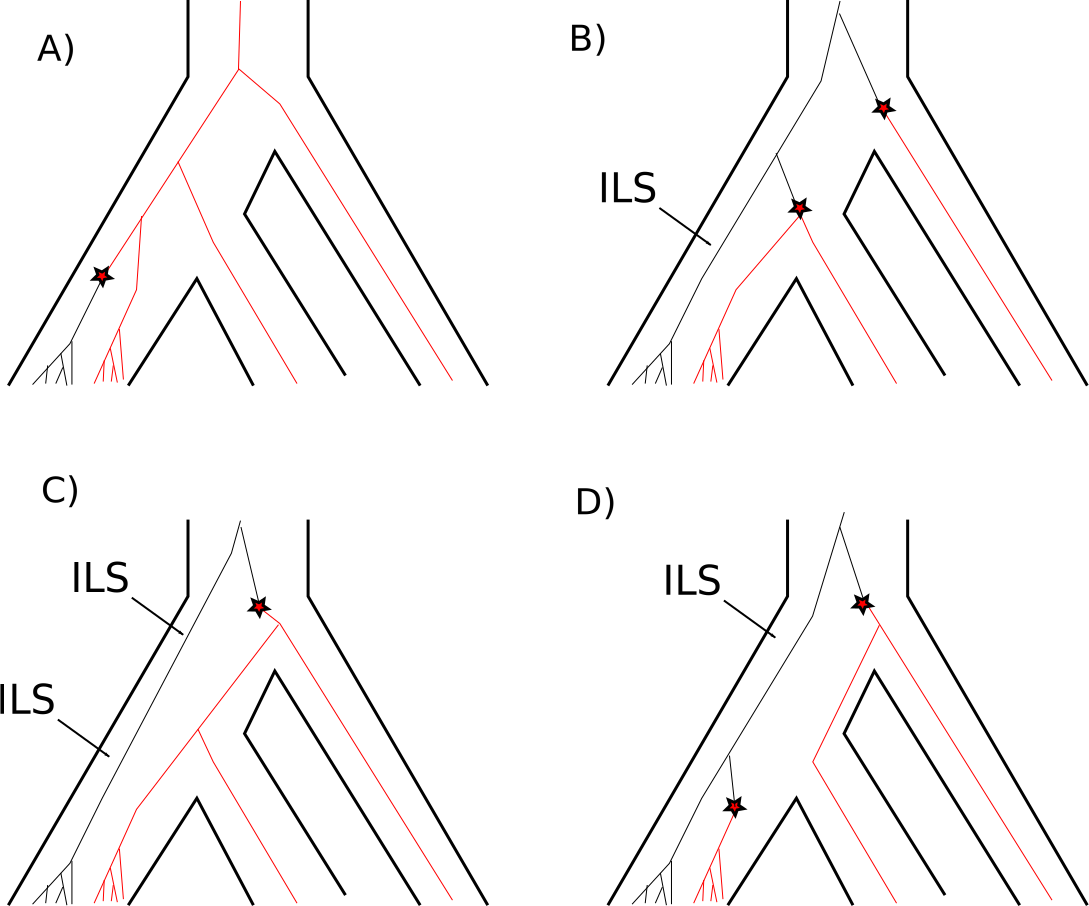
\includegraphics[width=\textwidth]{hcg-trees}
\end{center}
\vskip 2cm

We observe alleles that are polymorphic in humans (left branch),
and the same allele observed in one chimp (middle) and one gorilla (right).
Depicted are the four most parsimonious scenarios: 
in any case it requires one mutation;
and in other cases it requires at least two more rare(-ish) events:
incomplete lineage sorting (ILS) and/or another mutation.
The likelihoods are, I think:
\begin{align}
  p_A > p_B > p_C > p_D ,
\end{align}
(see below); but $D$ will create the bump on the right.

\begin{enumerate}

\item[A] The standard model, mutation sometime in the tree leading to modern humans.
Frequency distribution skewed towards low frequency.

\item[B] Two mutations, one leading to chimps and humans; the other on the gorilla lineage.  Requires the polymorphism in humans to be fairly old, so has a flat frequency distribution.

\item[C] One mutation, but long ago.  Requires the polymorphism to be old, again.

\item[D] Two mutations, one in chimp-gorilla and one in humans.  The red allele, being recently derived, has a skew towards low frequencies; which we miscall as high derived frequencies.

\end{enumerate}

\section{Asymmetric mutation}

Suppose possibly asymmetric mutation rates: $\muup$ from black to red,
and $\mudn$ from red to black.
Suppose that the probability of ILS in the whole human lineage is $\eta_C$,
and in the human-chimp ancestor is $\eta_G$.
Finally, suppose that the typical coalscence times in human, human-chip ancestor, and human-chimp-gorilla ancestor are, respectively, $T_H$, $T_C$, and $T_G$.
The the relative rates of $A$--$D$ are, roughly:
\begin{align}
A&: \mudn T_H & B&: \muup^2 T_C T_G \eta_C \\
C&: \muup T_G \eta_C \eta_G & D&: \muup^2 T_H T_G \eta_G  .
\end{align}

The human-chimp divergence is like 7 mya, 
and the human-chimp-gorilla only a couple more million years back;
and ancestral effective population sizes are thought to have been $\sim 10 \times$ larger than the human effective population size; so $\eta_G$ is not so small at all: 
like, 0.2?
On the other hand, we have lots of samples, so the chance of more than one lineage making it back to the human-chimp ancestor is pretty good, maybe of similar order?
If $\muup/\mudn \approx 10$, this suggests that the ratio of $A$ to $C$ is about 10:1.

In $C$ and $D$ the relevant numbers of generations for mutation should be around $10^5$; for $T_H$ in $D$ this is thanks to the large number of samples; 
and for $T_G$ in both this is thanks to the large effective population size of the ancestral population.  
Even if $\muup \approx 10^{-7}$, this still leaves $D$ about 1000 times less likely than $A$.

As for $B$, note that the mutation on gorilla has the full branch to occur on, i.e.~$\sim10^7$ years; so $\muup T_G$ is only a small factor.
Because there are fewer lineages to mutate, the mutation in human-chimp is less likely than the one occurring in $A$ by ad additional factor; and the incomplete lineage sorting is another factor. 
Incorporating $\muup/\mudn\approx10$, this suggest a $A:D$ ratio of only about 10:1.

%%%%%%%%
\section{Selection}

Selection (or biased gene conversion) will do several things:
effectively increase the mutation rate of the beneficial allele;
make ILS \emph{less} likely;
and distort the frequency spectrum.

\ldots effects on $A$--$D$?
\end{document}
